\documentclass[12pt]{article}

\usepackage{amsmath}
\usepackage{amssymb}
\usepackage{amsfonts}
\usepackage{geometry}
\usepackage{fancyhdr}
\usepackage{tikz}
\usepackage{amsthm}
\usetikzlibrary{calc,arrows.meta}

% Page setup
\geometry{margin=1in}
\setlength{\headheight}{15pt}
\pagestyle{fancy}
\fancyhf{}
\fancyhead[L]{Integrated Algebra 2 and Precalculus}
\fancyhead[R]{Assignment: Chapter 12 of Algebra 2}
\fancyfoot[C]{Page \thepage}

% Theorem environments
\newtheorem{definition}{Definition}
\newtheorem{theorem}{Theorem}
\newtheorem{example}{Example}
\newtheorem{lemma}{Lemma}

\begin{document}

\begin{center}
\textbf{\Large An Introduction to the Polar Coordinate System} \\
\vspace{0.5cm}
\makebox[0.4\textwidth]{Name: \enspace\hrulefill}
\hspace{0.1\textwidth}
\makebox[0.4\textwidth]{Date: \enspace\hrulefill}
\end{center}

\vspace{0.5cm}

\section{Introduction}

In our study of mathematics, we have primarily used the \textbf{Cartesian (or rectangular) coordinate system} to describe a point's position in a plane using horizontal and vertical distances $(x, y)$. While incredibly useful, it is not the only way. This chapter introduced the foundations of trigonometry, focusing on angles, degree measures, and the relationships between the sides of triangles. These tools allow us to build a different and powerful way of describing position: the \textbf{polar coordinate system}.

Instead of $(x,y)$ coordinates, the polar system uses a distance and an angle $(r, \theta)$ to locate a point. This approach is often far more convenient for describing objects and phenomena that have a natural center or rotational symmetry, such as planets orbiting a star, the radiation pattern of an antenna, or the elegant shapes of flowers. This assignment will introduce you to the fundamentals of polar coordinates, how they relate to the Cartesian system you already know, and how to graph beautiful and intricate curves using polar equations.

\section{Defining Polar Coordinates}

\begin{definition}
A point $P$ in the \textbf{polar coordinate system} is represented by an ordered pair $(r, \theta)$.
\begin{itemize}
    \item $r$ is the \textbf{directed distance} from a fixed point $O$, called the \textbf{pole} (or origin).
    \item $\theta$ is the \textbf{directed angle}, measured counterclockwise from a fixed ray called the \textbf{polar axis} to the segment $\overline{OP}$.
\end{itemize}
\end{definition}

\subsection{Converting Between Coordinate Systems}

The power of polar coordinates comes from their connection to trigonometry. By placing the pole at the origin of a Cartesian plane and aligning the polar axis with the positive x-axis, we can derive conversion formulas.

\begin{center}
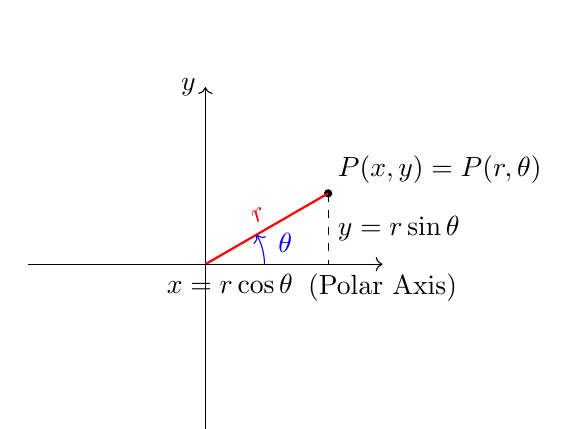
\begin{tikzpicture}[scale=1.5]
    % Axes
    \draw[->] (-1.5,0) -- (1.5,0) node[below] {$   \space    \space \text{(Polar Axis)}$};
    \draw[->] (0,-1.5) -- (0,1.5) node[left] {$y$};
    
    % Point P
    \coordinate (P) at (30:1.2);
    \fill (P) circle (1pt) node[above right] {$P(x,y) = P(r, \theta)$};
    
    % Lines to point
    \draw[thick, red] (0,0) -- (P) node[midway, above, sloped] {$r$};
    \draw[dashed] (P) -- (P |- 0,0) node[midway, right] {$y = r \sin\theta$};
    \draw[dashed] (0,0) -- (P |- 0,0) node[pos=0.2, below] {$x = r \cos\theta$};
    
    % Angle
    \draw[->, blue] (0.5,0) arc (0:30:0.5);
    \node[blue] at (15:0.7) {$\theta$};
\end{tikzpicture}
\end{center}

\begin{theorem}[Coordinate Conversion Formulas]
Let a point $P$ have Cartesian coordinates $(x,y)$ and polar coordinates $(r, \theta)$. Then:
\begin{align}
    \text{Polar to Cartesian:} \quad & x = r \cos\theta \quad \text{and} \quad y = r \sin\theta \\
    \text{Cartesian to Polar:} \quad & r^2 = x^2 + y^2 \quad \text{and} \quad \tan\theta = \frac{y}{x} \quad (\text{for } x \neq 0)
\end{align}
\end{theorem}

\begin{example}[Converting Coordinates]
\textbf{(a) Convert the polar point $(4, 30^\circ)$ to Cartesian coordinates.}
$$ x = 4 \cos(30^\circ) = 4 \left(\frac{\sqrt{3}}{2}\right) = 2\sqrt{3} $$
$$ y = 4 \sin(30^\circ) = 4 \left(\frac{1}{2}\right) = 2 $$
So the Cartesian coordinates are $(2\sqrt{3}, 2)$.

\textbf{(b) Convert the Cartesian point $(-3, 3)$ to polar coordinates.}
$$ r = \sqrt{(-3)^2 + 3^2} = \sqrt{9+9} = \sqrt{18} = 3\sqrt{2} $$
$$ \tan\theta = \frac{3}{-3} = -1 $$
Since the point $(-3,3)$ is in Quadrant II, we choose $\theta = 135^\circ$ or $\frac{3\pi}{4}$ radians. So a polar representation is $(3\sqrt{2}, 135^\circ)$.
\end{example}

\textit{Note:} Polar coordinates are not unique. The point $(3\sqrt{2}, 135^\circ)$ is also represented by $(3\sqrt{2}, -225^\circ)$ or even $(-3\sqrt{2}, 315^\circ)$. Why?

\section{Graphing Polar Equations}

Just as we graph equations like $y = x^2$ in the Cartesian plane, we can graph polar equations of the form $r = f(\theta)$. We can create a table of values $(\theta, r)$ and plot the points.

\begin{example}[Graphing a Cardioid]
Sketch the graph of the polar equation $r = 2 + 2\cos\theta$.

We can test some values for $\theta$:
\begin{center}
\begin{tabular}{|c|c|c|c|c|c|}
\hline
$\theta$ & $0^\circ$ & $60^\circ$ & $90^\circ$ & $120^\circ$ & $180^\circ$ \\
\hline
$\cos\theta$ & 1 & 0.5 & 0 & -0.5 & -1 \\
\hline
$r = 2+2\cos\theta$ & 4 & 3 & 2 & 1 & 0 \\
\hline
\end{tabular}
\end{center}
By plotting these and other points, we get a heart-shaped curve called a \textbf{cardioid}.
\end{example}

\newpage

\section{Practice Problems}

\textbf{Part A: Basic Conversions and Plotting}

\textbf{1.} Plot the following polar coordinates on a polar grid:
\begin{enumerate}
    \item[(a)] $(3, 45^\circ)$
    \item[(b)] $(5, 120^\circ)$
    \item[(c)] $(2, -60^\circ)$
    \item[(d)] $(-4, 150^\circ)$
\end{enumerate}
\vspace{4cm}

\textbf{2.} Convert the following polar coordinates to Cartesian coordinates.
\begin{enumerate}
    \item[(a)] $(6, 30^\circ)$
    \vspace{2cm}
    \item[(b)] $(4, \frac{3\pi}{4})$
    \vspace{2cm}
    \item[(c)] $(-2, 210^\circ)$
    \vspace{2cm}
\end{enumerate}

\textbf{3.} Convert the following Cartesian coordinates to polar coordinates. Give one answer with $r>0$ and $0^\circ \leq \theta < 360^\circ$.
\begin{enumerate}
    \item[(a)] $(5, 5)$
    \vspace{2cm}
    \item[(b)] $(-4, 4\sqrt{3})$
    \vspace{2cm}
    \item[(c)] $(0, -3)$
    \vspace{2cm}
\end{enumerate}

\textbf{Part B: Graphing Polar Equations}

\textbf{4.} Convert the rectangular equation to a polar equation. Simplify your answer.
\begin{enumerate}
    \item[(a)] $x^2 + y^2 = 25$
    \vspace{3cm}
    \item[(b)] $y = 5$
    \vspace{3cm}
\end{enumerate}

\textbf{5.} Convert the polar equation to a rectangular equation.
\begin{enumerate}
    \item[(a)] $r = 4\sec\theta$
    \vspace{3cm}
    \item[(b)] $r = \frac{6}{2\cos\theta - 3\sin\theta}$
    \vspace{3cm}
\end{enumerate}

\textbf{6.} Sketch the graph of the polar equation $r=4\sin\theta$ by first completing a table of values for $\theta = 0, \frac{\pi}{6}, \frac{\pi}{4}, \frac{\pi}{3}, \frac{\pi}{2}$. What shape is it?
\vspace{6cm}

\textbf{Part C: Advanced Applications}

\textbf{7.} Identify and sketch the graph of the polar equation $r = 3 - 3\cos\theta$.
\vspace{6cm}

\textbf{8.} A rose curve is given by an equation of the form $r = a \cos(n\theta)$ or $r=a\sin(n\theta)$.
\begin{enumerate}
    \item[(a)] Sketch the graph of the rose curve $r = 4\cos(2\theta)$. How many petals does it have?
    \vspace{5cm}
    \item[(b)] Sketch the graph of the rose curve $r = 4\cos(3\theta)$. How many petals does it have?
    \vspace{5cm}
    \item[(c)] Make a conjecture about the number of petals of $r = a\cos(n\theta)$ when $n$ is even versus when $n$ is odd.
    \vspace{2cm}
\end{enumerate}

\textbf{9.} \textbf{Challenge Problem:} The distance $d$ between two points with polar coordinates $(r_1, \theta_1)$ and $(r_2, \theta_2)$ can be found using the Law of Cosines on the triangle formed by the pole and the two points. The formula is:
$$d = \sqrt{r_1^2 + r_2^2 - 2r_1r_2\cos(\theta_2 - \theta_1)}$$
Find the distance between the points $(3, 60^\circ)$ and $(5, 150^\circ)$.
\vspace{5cm}

\end{document}
